\section{Recommendations}

\subsection {Solution To Challenge 1: Structuring Requirements}

Instead of following the trial and error process to refine formalized requirements in ways to verify that requirement, we tried to address this issue at its root cause - the requirement document. The system behaviors of control systems are typically grouped in terms of \emph{modes} - a logical way to describe a set of system behaviours. In a complex system, there could be many such modes and they could either be mutually exclusive (only one mode can be active at a time) or orthogonal (multiple modes can be active at a time). Lucent understanding of such modes and their groups was crucial to systematically formalize the requirements. In the GPCA, there were three main orthogonal groups of modes - infusion, alarm and configuration. Within each orthogonal group, there were a set of modes that were mutually exclusive of each other. For instance, within infusion mode group basal, intermittent and patient bolus modes are mutually exclusive to each other. Similarly, in the alarm group, each each exceptional condition was considered mutually exclusive to each other. We decided to leverage this pattern of modes and use it to organize requirement statements in the the requirements document.

 \begin{figure}[h!]
    \centering
    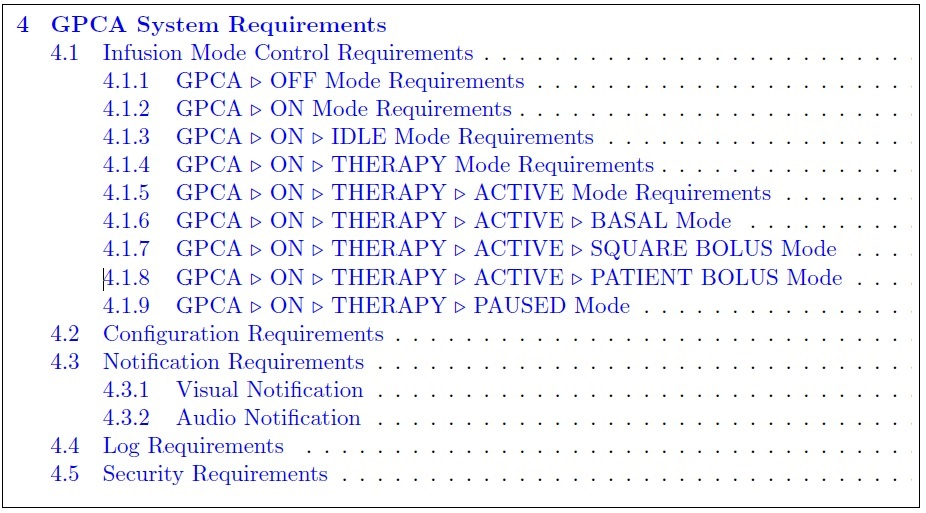
\includegraphics[width=\columnwidth]{images/structuring.jpg}
    \caption{GPCA System Requirements Structuring}
    \label{fig:gpca-requirements}
 \end{figure}

We restructured the requirement document and followed a hierarchical structure to organize requirements of the GPCA, as shown in Figure~\ref{fig:gpca-requirements} that not only simplified the formalization process, but also brought about conceptually clarity of the requirements. In this structure, the requirements that were common to the entire system, irrespective of the modes, such as startup behavioural requirements were placed at the top of the hierarchy. At the second level in the hierarchy, we placed the three mode groups - infusion, alarm and configuration - that indicated the orthogonality among them. Within each orthogonal mode group, we again followed the hierarchical structure to organize their requirements. The infusion mode group had three mutually exclusive modes - basal, intermittent bolus and patient bolus. While documenting their requirements, we observed that there were only a few requirements that were specific to each of those infusion modes whereas several requirements were common to all of them. To avoid repetition of requirements, we grouped all the common requirements to a parent mode called ``therapy", and then organized the three infusion modes as its child modes with specific requirements.

 \begin{figure}[h!]
    \centering
    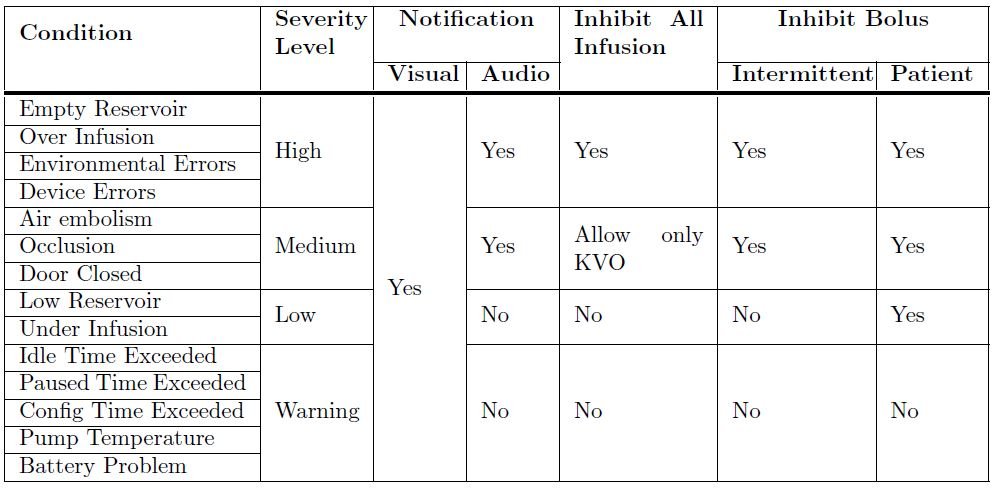
\includegraphics[width=\columnwidth]{images/alarm.jpg}
    \caption{Notification Requirements Table}
    \label{fig:gpca-alarm}
 \end{figure}

Within the alarm group, we identified four 4 levels of severity by grouping common system responses described for each condition. We conceptualized the severity level category as parent modes and each condition with them as child modes. This allowed us to categorize the 18 individual conditions within one of the four levels and organize their requirements within the respective severity level. For example, all highest severity conditions caused the system to raise audio alarm, display error message and stop infusion, whereas all low severity level conditions caused the system to display an error message. Although we came across a couple of conditions whose requirements that did not exactly match the requirements of the four groups, we were able to negotiate with our domain experts to match the differences. To make the documentation clear, we used a table to document the conditions and the expected system responses, as shown in Figure~\ref{fig:gpca-alarm}.

This structuring greatly helped in systematically formalize each requirement. It helped provide enough information about the orthogonality and exclusivity among the modes. Infact, in some cases it helped identify and raise the right questions to discover missing or clarify ambiguous requirements. We were able to refer to the requirements document and formalize the requirements in a straightforward fashion, that otherwise would have been a ardours trial and error approach. For instance, by examining the requirements hierarchically from the top level, we were able to systematically identify that the precise formalization of the patient infusion requirement includes the operating condition of the system (whether the system is ON/OFF) and its orthogonal alarm requirements to systematically identify exceptional conditions that avoids infusion and vice versa. This structuring significantly reduced the effort to arrive at the precise formalization. %Another significant benefit of this structuring is the clarity it provides in documenting the mode transition requirements within infusion modes - descriptions about how and when transitions between those modes occur. We documented the requirements on transitions between the three modes within therapy mode, its immediate parent mode. This strategy allowed us to systematically formalize and verify the mode transition requirements -- a common source of problem in modal systems.
For example, the formalized requirements for patient bolus infusion was:
\\\\
\footnotesize{\texttt{
SystemOn~and~not(InfusionInhibitAlarms) and \\ \textcolor{white}{---}not(Configuring)~and~(PatientRequest)~$\Rightarrow$ \\
\textcolor{white}{--------}SoftwareFlowRate~=~PatientFr}}
\\\normalsize{}\\

Similarly, formalizing the alarm requirements to verify them individually also became straightforward. Grouping the exceptional conditions and its associated actions in the requirements document eased the process of formalizing the requirements. We used variables (or macros) to capture the conditions that cause that alarm level and the desired actions, to avoid repetition in definitions. It then became systematic and straightforward to individually check a requirement. For example, in the GPCA there were 3 exceptional conditions that we categorized as medium level alarms, namely air in line (sensor input indicating air in infusion tube), occlusion (sensor input indicating blockage in infusion tube) and door open (sensor input indicating drug reservoir enclosure is opened). To check the door open requirement exclusively, we systematically excluded the all higher priority level alarm (HiLevelAlarm is a logical disjunction of all conditions within the highest severity level) and the other conditions in its peer level, as shown below :
\\\\
\footnotesize{\texttt{SystemOn and not(HiLevelAlarm) and \\
\textcolor{white}{----}not(AirInLine) and not(Occlusion) and \\ \textcolor{white}{------}(DoorOpen)$\Rightarrow$\\
\textcolor{white}{--------} MedLevelAlarmActions}}
\\\normalsize{}

While such hierarchical structuring is common when trying to model the system or developing source code, it has not be widely used to document requirements in the requirements engineering community. %We found that using such a strategy not only helps organize requirement in a conceptually clear manner, but significantly reduces the effort for formalizing requirements and avoids errors in the process. 

\subsection {Solution For Challenge 2: Richer Traceability}

When we identified this issue for one requirement, we started documenting the traceability between the system and software requirements. In addition to mapping each system requirement to the corresponding software requirement, we also documented an argument (as semiformal statements) explaining how the software requirement contributes to satisfying the system level requirement. While the original intent to document this richer traceability was to establish a satisfaction argument between requirements at different levels of abstraction, it actually helped us to understand the precise role of each component to satisfy the system requirement. In fact, by documenting this type of richer traceability we were able to identify 10 incorrectly formalized software requirements out of the 86 system level requirements of the GPCA. In sum, documenting a richer traceability clarified the role of each component requirement in satisfying the system level requirement and the helps identify the mathematical difference between capturing them - one of the pitfalls in formal verification.

\anitha{I want to put a figure from the traceability document for this requirement here.}

\subsection {Solution For Challenge 3: Sanity Checks and Fallibility Detection}

We believe that the root cause of this problem was not the tool's default setting, but the fact that it was not apparent. Hence, to address the issue from the tool side we requested the tool developers to provide elaborate messages of certain key configurations when using the features. After the change, AGREE now displays the depth of check along with the result of consistency checking. While such a change may not be possible with every tool and feature we use, we strongly recommend the engineers to delve deep into the details and configuration of tool to precisely understand the results, especially when there is limited information provided by the tool along with the results.

\subsection {Solution For Challenge 4: Automating Verifiers}

\anitha{I need to write a little about the tools above helps identify these issues + need translators and rigours process}